
\section{Sequence Alignment}

The comparison of two or more sequences, measuring the extent to which they differ, is important in many scientific areas, most notably in molecular biology~\cite{needleman70,smith81,carrillo88,wang94} where it has been critical
in the understanding of functional, structural, or evolutionary relationships between the sequences~\cite{kruskal83,mount05book}.

A particularly important comparison technique is sequence alignment, which identifies a series of patterns that appear in the same order in the sequences.
Essentially, sequence alignment algorithms insert blank characters in both input sequences so that the final sequences end up having the same size, where equivalent segments are aligned with their matching segments from the other sequence and non-equivalent segments are either paired with the blank or a mismatching character.

Figure~\ref{fig:seq-align-example} shows an example of a pair-wise sequence alignment.
This example, adapted from Lee~et~al.~\cite{lee02}, shows two protein sequences where amino acids are represented by their one-letter symbology~\cite{aasland68}.

\begin{figure}[h]
  \centering
  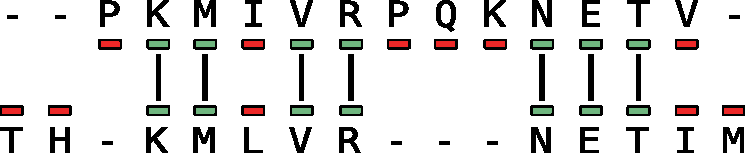
\includegraphics[scale=0.55]{src/background/figs/seq-align-example}
  \caption{Example of an optimum alignment between two sequences.
  Matching segments are shown in green, vertically centred, and the non-matching segments are shown in red at the sides.}
  \label{fig:seq-align-example}
\end{figure}

Formally, sequence alignment can be defined as follows:
For a given alphabet $\alpha$, a sequence $S$ of $k$ characters is an element of
$\alpha^k$, i.e., $S = (a_1, \ldots a_k)$.
Let $S_1, \ldots, S_m$ be a set of sequences, possibly of different lengths but
all derived from the same alphabet $\alpha$, where
$S_i = (a_1^{(i)}, \ldots, a_{k_i}^{(i)})$, for all $i\in\{1,\ldots,m\}$.
Consider an extended alphabet that includes the \textit{blank} character ``$-$'',
i.e., $\beta = \alpha \cup \{-\}$.
An alignment of the $m$ sequences, $S_1, \ldots, S_m$, is another set of sequences,
$\bar{S}_1, \ldots, \bar{S}_m$, such that each sequence $\bar{S}_i$ is obtained
from $S_i$ by inserting blanks in positions where some of the other sequences
have non-blank and possibly equivalent characters, for a given equivalence relation.
All sequences $\bar{S}_i$ in the alignment set have the same length $l$, where
$\max\{k_1,\ldots,k_m\} \leq l \leq k_1 + \cdots + k_m$.
Moreover, $\forall i\in\{1,\ldots, m\}$, $\bar{S}_i = (b_1^{(i)},\ldots,b_l^{(i)})$,
there are increasing functions $v_i: \{1,\ldots,k_i\} \to \{1,\ldots,l\}$, such that:
\begin{itemize}
\item $b_{v_i(j)}^{(i)} = a_j^{(i)}$, for every $j \in \{1,\ldots,k_i\}$;
\item any position not covered by the function $v_i$ contain a black character, i.e., for every $j \in \{1,\ldots,l\}\setminus \textrm{Im} \, v_i$, $b_j$ is the blank character ``$-$''.
\end{itemize}
Finally, for all $j\in\{1,\ldots,l\}$, there is at least one value of $i$ for which $b_j^{(i)}$ is not a blank character.
Note that two aligned sequences may contain both non-blank and non-equivalent characters at any given position, in which case there is a mismatch.

The sequence alignment problem is concerned with identifying an alignment that maximises the score for a given scoring scheme.
The scoring scheme first defines a weight for the alignment of pairs of characters which will then be used to compose a score for the whole sequence alignment.
These weights are used to penalise mismatches and gaps while favouring matching pairs.

The alignment score between two characters is defined by a function on pairs of characters, $\delta \in \beta\times\beta \to \mathbb{R}$, for a given extended alphabet $\beta$.
The simplest function that is commonly used is the constant function~\cite{haque09}.
Let $a,b\in\beta$ and $a \neq b$.
This constant function is defined by a triple $(w_1,w_2,w_3)\in\mathbb{R}^+\times\mathbb{R}^-\times\mathbb{R}^-$, such that:
\begin{itemize}
\item For two matching caracters, $\delta(a,a) = w_1, w_1\in\mathbb{R}^+$.
\item For a mismatch betweem non-blank characters, $\delta(a,b) = w_2, w_2\in\mathbb{R}^-$.
\item The gap penalty, for when we have a blank character, $\delta(a,-) = \delta(-,a) = w_3, w_3\in\mathbb{R}^-$.
\end{itemize}
This is a simple scoring scheme that rewards matches and penalises mismatches and gaps.

There is a vast literature on algorithms for performing sequence alignment, especially in the context of molecular biology.
These algorithms are classified as either global or local.
A global sequence alignment algorithm attempts to align the entire sequence, using as many characters as possible, up to both ends of each sequence.
Global alignment algorithms are useful for sequences that are highly similar and have approximately the same length~\cite{mount05book}.
Alternatively, a local sequence alignment algorithm generates subalignments in stretches of sequence with the highest density of matches.
Local alignments are more suitable for aligning sequences with very few similarities or vastly different lengths~\cite{mount05book}.

In this work, we will focus on pair-wise global alignment algorithms.
The following sections describe the main optimal algorithms based on dynamic programming.
These algorithms will offer different optimality, performance, and memory usage trade-offs~\cite{needleman70,smith81,carrillo88,hickey11}.
%Different alignments would produce different but valid merged functions.

\subsection{Needleman-Wunsch Algorithm}

The Needleman-Wunsch algorithm~\cite{needleman70} is one of the most well known algorithm for pair-wise global alignment.
This algorithm gives an alignment that is guaranteed to be optimal for a given scoring scheme~\cite{higgins89}.

The Needleman-Wunsch algorithm is based on dynamic programming and consists of two main steps.
First, it builds a \textit{similarity matrix}, based on a scoring scheme, which assigns weights for matches, mismatches, and \textit{gaps} (blank characters).
Afterwards, a backward traversal is performed on the similarity matrix, in order to reconstruct the final alignment by maximizing the total score.

\begin{figure}[h]
  \centering
  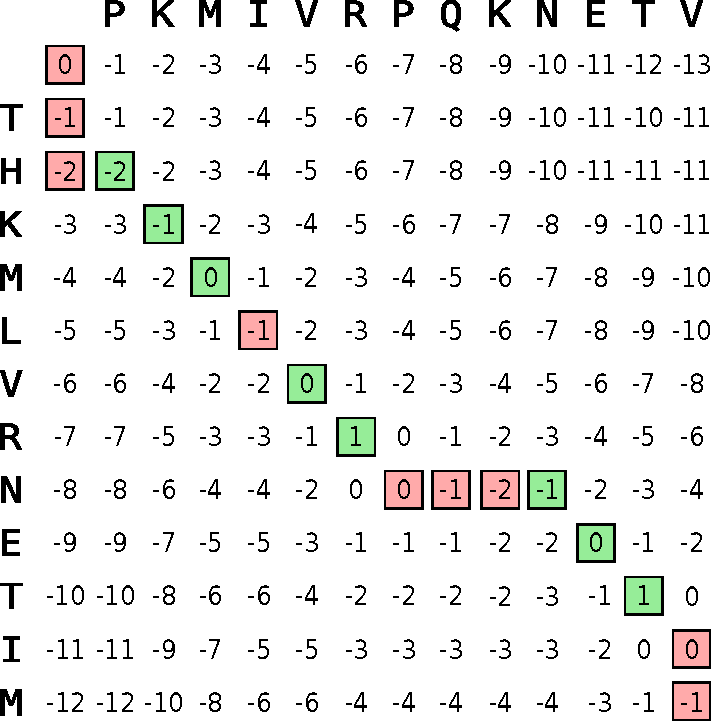
\includegraphics[scale=0.6]{src/background/figs/seq-align-example-nw}
  \caption{.}
  \label{fig:seq-align-example-nw}
\end{figure}

Figure~\ref{fig:seq-align-example-nw} shows the similarity matrix corresponding to the example from Figure~\ref{fig:seq-align-example}.
The similarity matrix is constructed by comparing all possible pairs of characters from the input sequences.
Let $S_1$ and $S_2$ be our input sequences of sizes $k_1$ and $k_2$, respectively, where $S_1 = (a_1,\ldots,a_{k_1})$ and $S_2 = (b_1,\ldots,b_{k_2})$.
The similarity matrix $M$ computed for these two input sequences will have size $(k_1 + 1) \times (k_2+1)$.
Let $M_{i,j}$ denote all entries in the similarity matrix, with $1 \leq i \leq (k_1 + 1)$ and $1 \leq j \leq (k_2 + 1)$.
The first entry in the matrix is $M_{1,1} = 0$, and
\begin{equation*}
%\begin{align*}
M_{i,j} = \max \begin{cases}
  M_{i-1,j} + \delta(a_{i-1},-)         &  \quad  \text{if } i>1 \text{ and } j\geq1 \\
  M_{i,j-1} + \delta(-,b_{j-1})         &  \quad  \text{if } i\geq1 \text{ and } j>1 \\
  M_{i-1,j-1} + \delta(a_{i-1},b_{j-1}) &  \quad  \text{if } i>1 \text{ and } j>1
\end{cases}
%\end{align*}
\end{equation*}
In other words, the score for each cell in the similarity matrix is the maximum among the rules shown in Figure~\ref{fig:seq-align-rules}.

\begin{figure}[h]
  \centering
  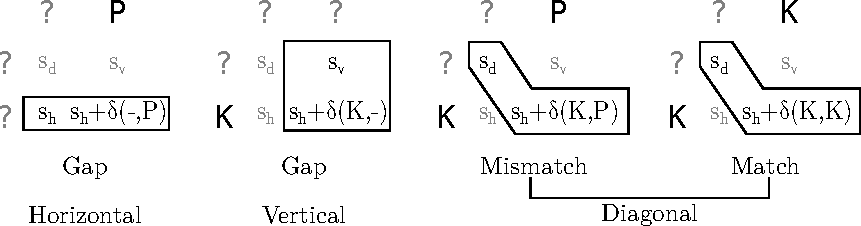
\includegraphics[scale=0.8]{src/background/figs/seq-align-rules}
  \caption{.}
  \label{fig:seq-align-rules}
\end{figure}


Figure~\ref{fig:seq-align-example-nw} also highlights the traversal. 
Note that sometimes, while traversing the score matrix, there are multiple adjacent neighbours with the same score.
Since there may exist multiple traversals with the same score, two sequences can have multiple optimum alignments.

Needleman-Wunsh algorithm is quadratic in the size of the sequences being aligned, both in time and space.

\subsection{Hirschberg Algorithm}
